\documentclass[a4paper,10pt, twocolumn]{article}

\usepackage{float}
\usepackage{graphicx}
\usepackage{caption}
%\usepackage{subcaption}
%\usepackage{pdfpages}
\graphicspath{{../../results/}}

\begin{document}
\section{Are EnTrI results biased?}
Since transposon insertion biases can affect the essentiallity level inferred from transposon mutagenesis experiments, the dataset has been tested for two types of biases: the distance from the origin and GC content.
% As Figure~\ref{fig:distance_bias} shows, there is an insertion index bias towards the position of the genes for different strains.
The distance bias in every individual strain is depicted in Figure~\ref{fig:distance_bias_individual}. These plots indicate that the bias is negligible in some strains like Salmonella typhi, while the insertion indices of the genes in other strains need to be normalised by their distances from the origin. We have used the LOESS curve and for each strain, divided the insertion indices by the predicted LOESS value to normalise the insertion indices. As the distribution of new insertion indices will be around 1, we have multiplied the resulted values by the mean of the initial insertion indices to have a distribution around the mean. The results are shown in Figure~\ref{fig:normalised_distance_bias}.

%\begin{figure}[H]
%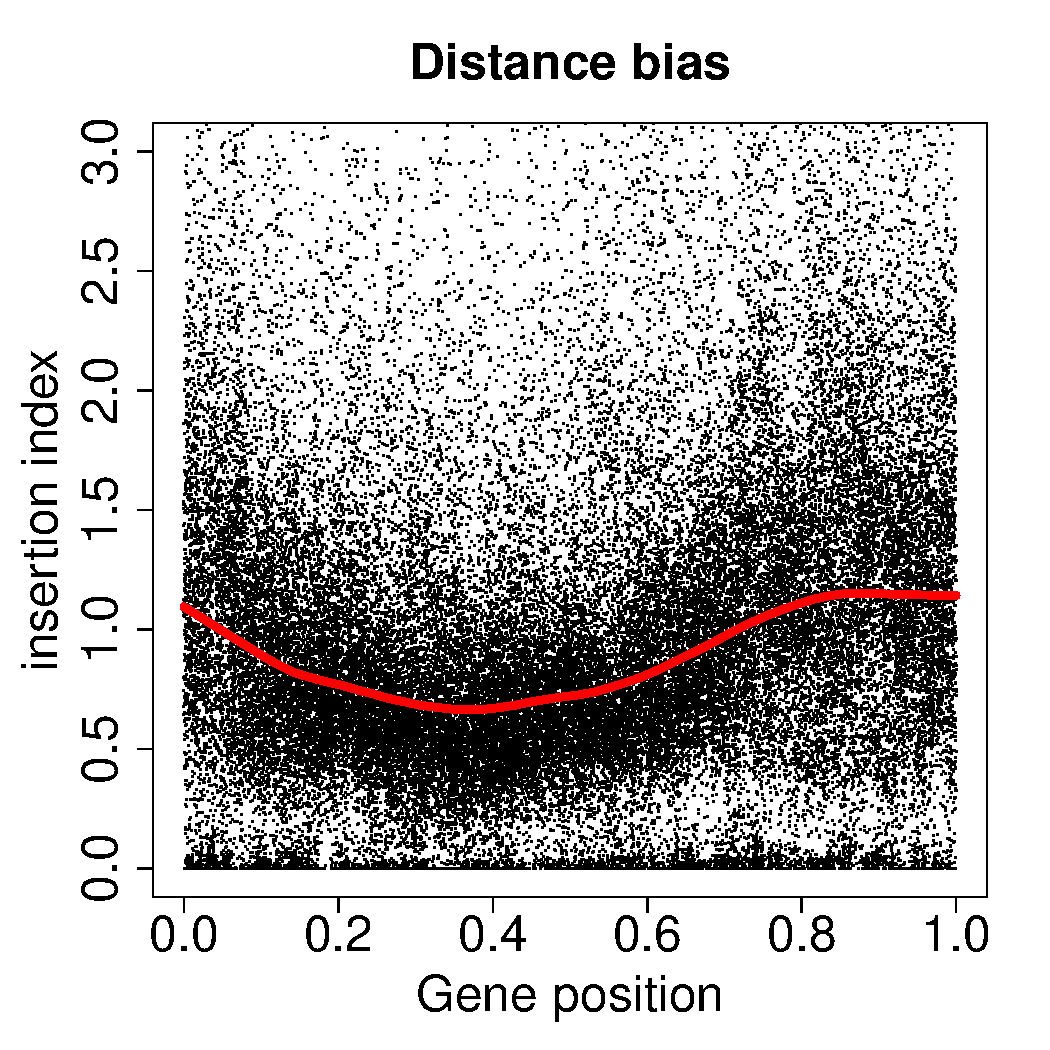
\includegraphics[scale=0.28, page=1]{biases.pdf}
%\caption{The bias towards the distance from origin (DnaA gene) for all of the species under study. The red curve shows the fitted LOWESS regression curve.}
%\label{fig:distance_bias}
%\end{figure}

\begin{figure*}
\centering
\begin{tabular}{c c c}
\includegraphics[page=2, scale=0.22]{biases.pdf} & 
\includegraphics[page=4, scale=0.22]{biases.pdf} &
\includegraphics[page=6, scale=0.22]{biases.pdf} \\
\includegraphics[page=8, scale=0.22]{biases.pdf} & 
\includegraphics[page=10, scale=0.22]{biases.pdf} &
\includegraphics[page=12, scale=0.22]{biases.pdf} \\
\includegraphics[page=14, scale=0.22]{biases.pdf} & 
\includegraphics[page=16, scale=0.22]{biases.pdf} &
\includegraphics[page=18, scale=0.22]{biases.pdf} \\
\includegraphics[page=20, scale=0.22]{biases.pdf} & 
\includegraphics[page=22, scale=0.22]{biases.pdf} &
\includegraphics[page=24, scale=0.22]{biases.pdf}
\end{tabular}
\caption{The bias towards the position of the gene for every individual strain. The red curves show the fitted LOESS curves.}
\label{fig:distance_bias_individual}
\end{figure*}

\begin{figure*}
\centering
\begin{tabular}{c c c}
\includegraphics[page=3, scale=0.22]{biases.pdf} & 
\includegraphics[page=5, scale=0.22]{biases.pdf} &
\includegraphics[page=7, scale=0.22]{biases.pdf} \\
\includegraphics[page=9, scale=0.22]{biases.pdf} & 
\includegraphics[page=11, scale=0.22]{biases.pdf} &
\includegraphics[page=13, scale=0.22]{biases.pdf} \\
\includegraphics[page=15, scale=0.22]{biases.pdf} & 
\includegraphics[page=17, scale=0.22]{biases.pdf} &
\includegraphics[page=19, scale=0.22]{biases.pdf} \\
\includegraphics[page=21, scale=0.22]{biases.pdf} & 
\includegraphics[page=23, scale=0.22]{biases.pdf} &
\includegraphics[page=25, scale=0.22]{biases.pdf}
\end{tabular}
\caption{The insertion indices are normalised by the predicted LOESS value and the mean of the insertion indices. The red curves show the fitted LOESS curves.}
\label{fig:normalised_distance_bias}
\end{figure*}

We have also checked for GC bias. There was a bias towards the GC content of the genes and we normalised the insertion indices for GC content in the same way as we did for gene position. The results, before and after the normalisation, are plotted in Figure~\ref{fig:GC_bias}. To see if there is any positional bias for any nucleotide, the nucleotides around the insertion sites (the insertion site and 10 nucleotides on each side) are stacked on top of each other and a sequence logo is generated from these sequences. It can be inferred from Figure~\ref{fig:logo} that there is no significant bias in any position. 

\begin{figure*}
\centering
\begin{tabular}{c c}
\includegraphics[scale=0.35, page=26]{biases.pdf} &
\includegraphics[scale=0.35, page=27]{biases.pdf}
\end{tabular}
\caption{The bias towards GC content. The LOESS curve is shown in red.}
\label{fig:GC_bias}
\end{figure*}

\begin{figure}
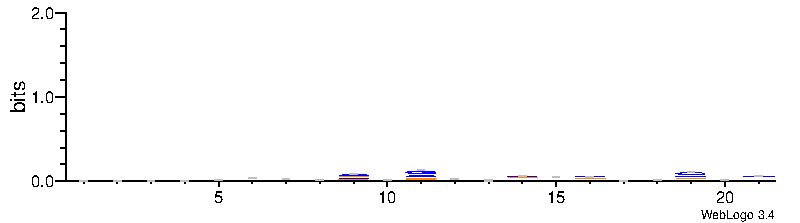
\includegraphics[scale=.98, angle = -90]{logo.pdf}
\caption{The nucleotides around the insertion sites (the insertion site and 10 nucleotides on each side) are stacked on top of each other and a sequence logo is generated from these sequences using webLogo stand-alone package. The height of the letter stack in each position shows how conserved the bases in that position are.}
\label{fig:logo}
\end{figure}

\section{Can we recover phylogenetic information from the essential genes?}
To get the evolutionary relationship among all our strains, we collected all clusters with one and only one gene per genome and concatenated all the genes corresponding to every strain. Then aligned them using mafft and generated a phylogenetic tree using fasttree software. The resulted phylogenetic tree is depicted in Figure~\ref{fig:species-tree}.

\begin{figure}
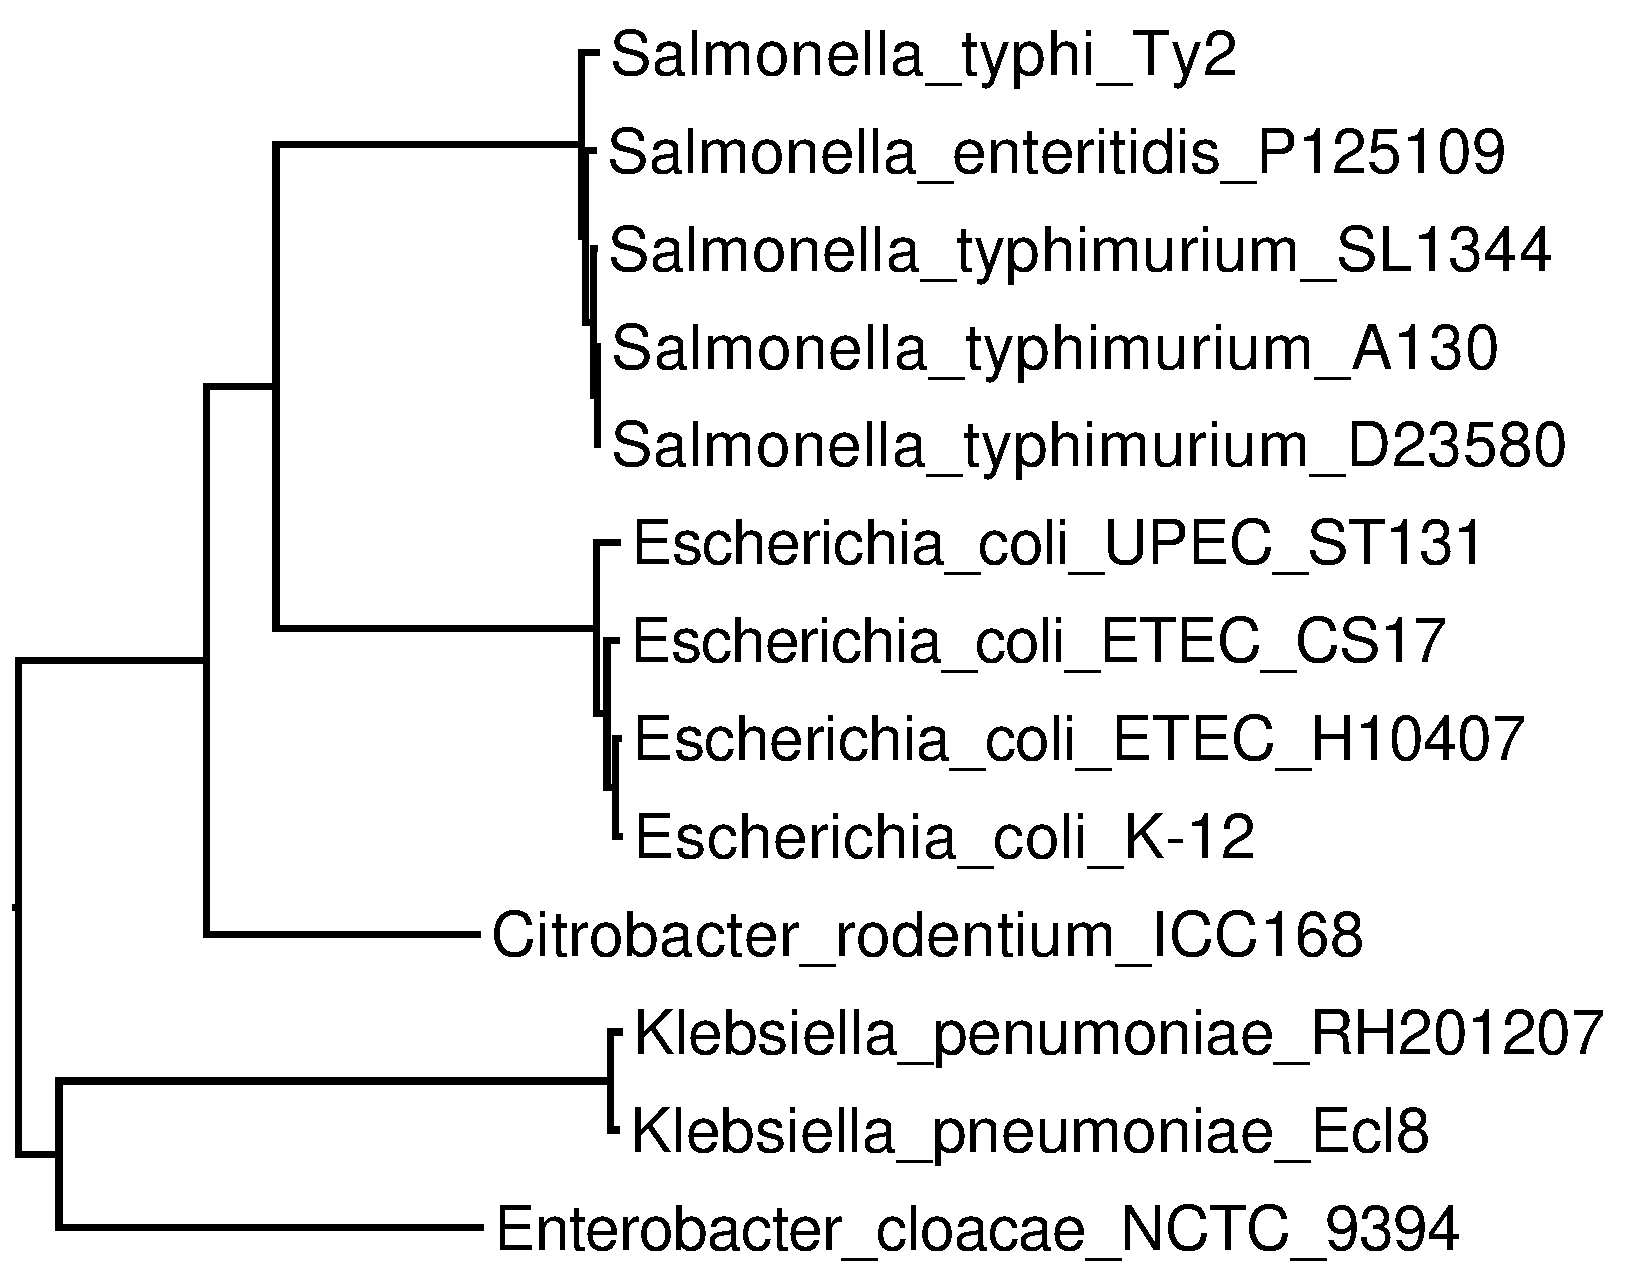
\includegraphics[scale=0.14]{../speciestree/speciestree.pdf}
\caption{The tree is generated from all the clusters with one and only one gene per strain.}
\label{fig:species-tree}
\end{figure}

To test if the same tree can be obtained from the essentiality of genes, we have selected all clusters that contain exactly one gene from each strain (82 clusters) and made a binary matrix from the essentiality of the genes in these clusters. If a gene is essential in a strain, the corresponding value in the matrix is 1 and if the gene  is not essential, the value is 0. Then, we have generated a distance matrix from these values using Bray-Curtis distance and plotted a phylogenetic tree.  Figure~\ref{fig:essentiality-tree} indicates that the resulting tree does not maintain the phylogenetic information of the species under study.

\begin{figure}
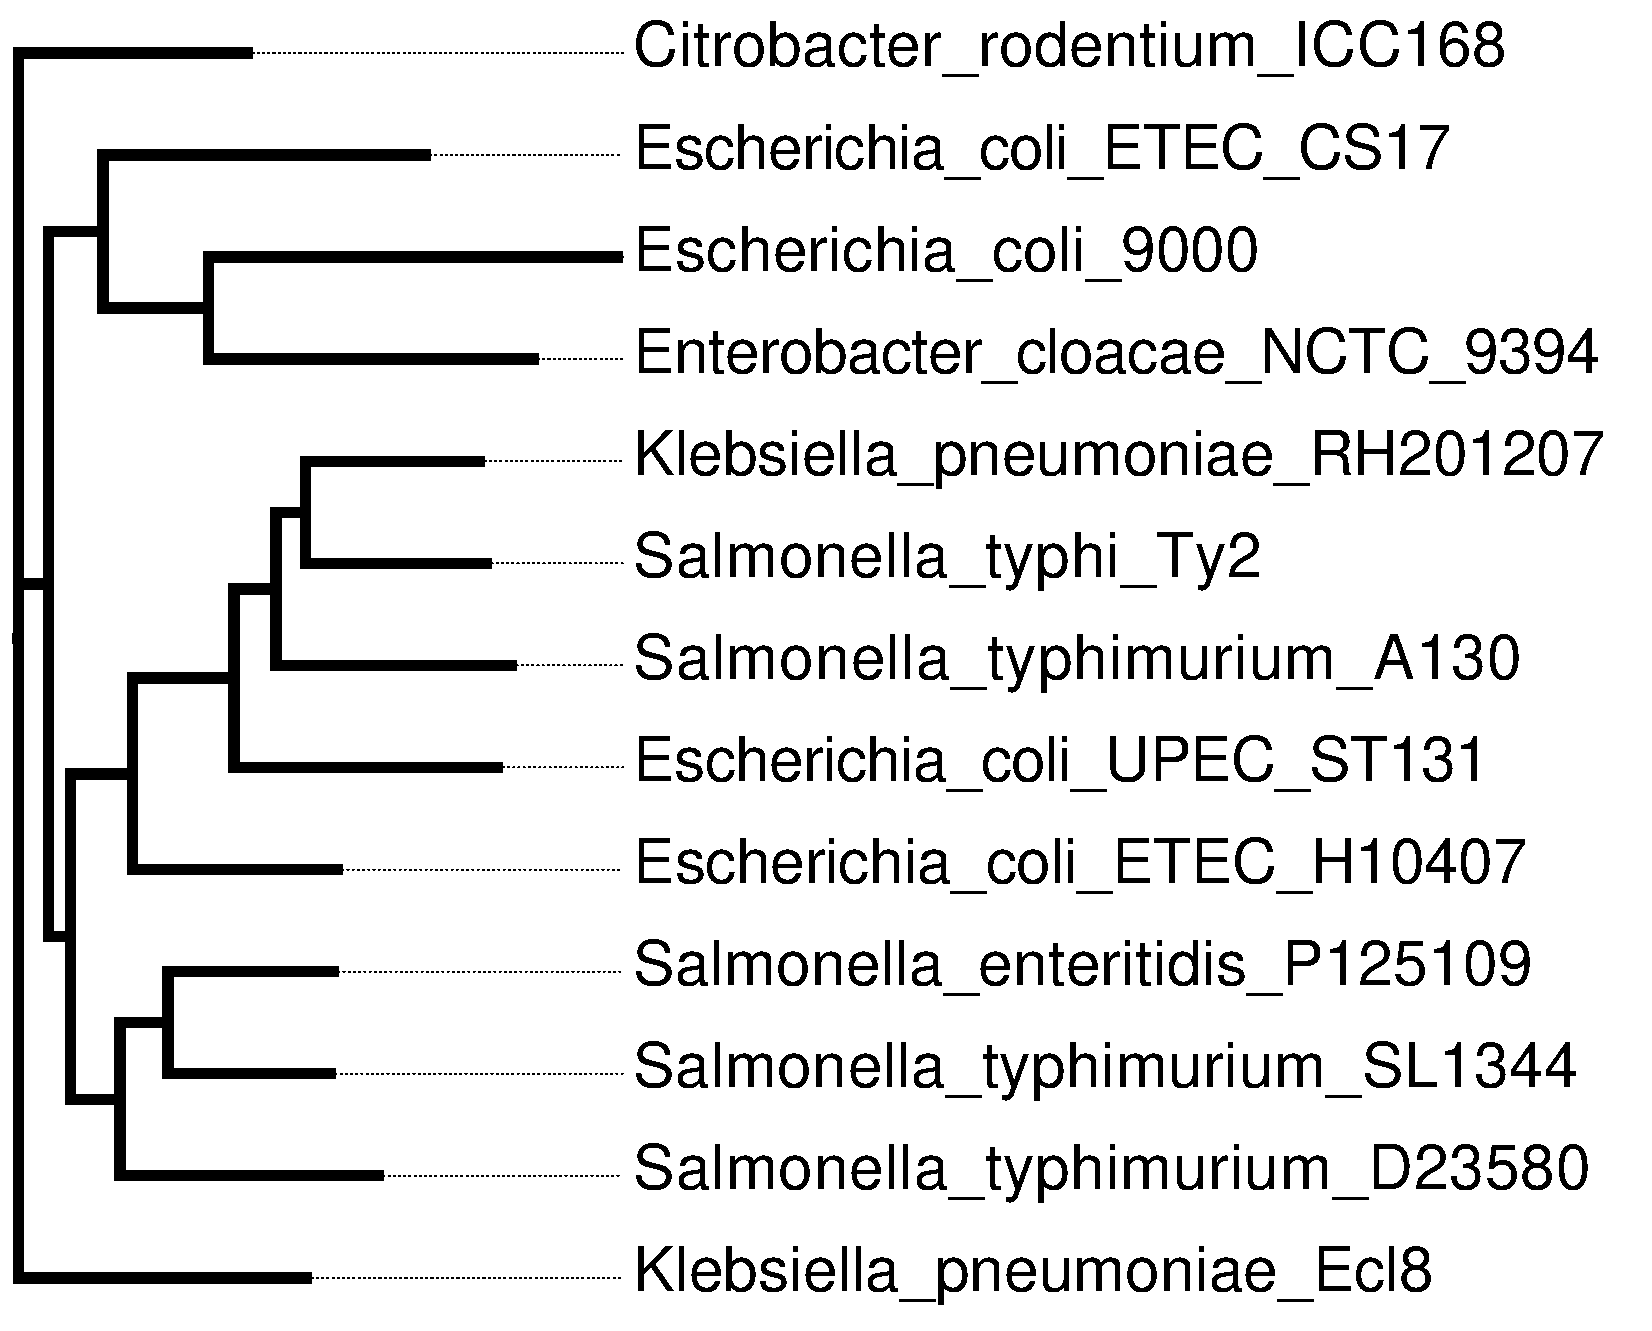
\includegraphics[scale=0.14]{make-essentiality-tree/essentiality-tree.pdf}
\caption{The phylogenetic tree is generated using ``phylip neighbor'' software.}
\label{fig:essentiality-tree}
\end{figure}

We have also compared every pair of strains and calculated the number of genes that are essential in one strain and absent in the other, the number of genes that are essential in both strains, the number of genes that are essential in one strain and present but not essential in the other strain, the number of genes that are present in one strain and absent in the other, and the number of genes that are shared between the two strains. The resulted heatmaps can be seen in Figure~\ref{fig:pairwise-venn}. The dendograms obtained from heatmaps in this figure are consistent with the species tree to some extent. 

\begin{figure*}
\centering
\begin{tabular}{c c}
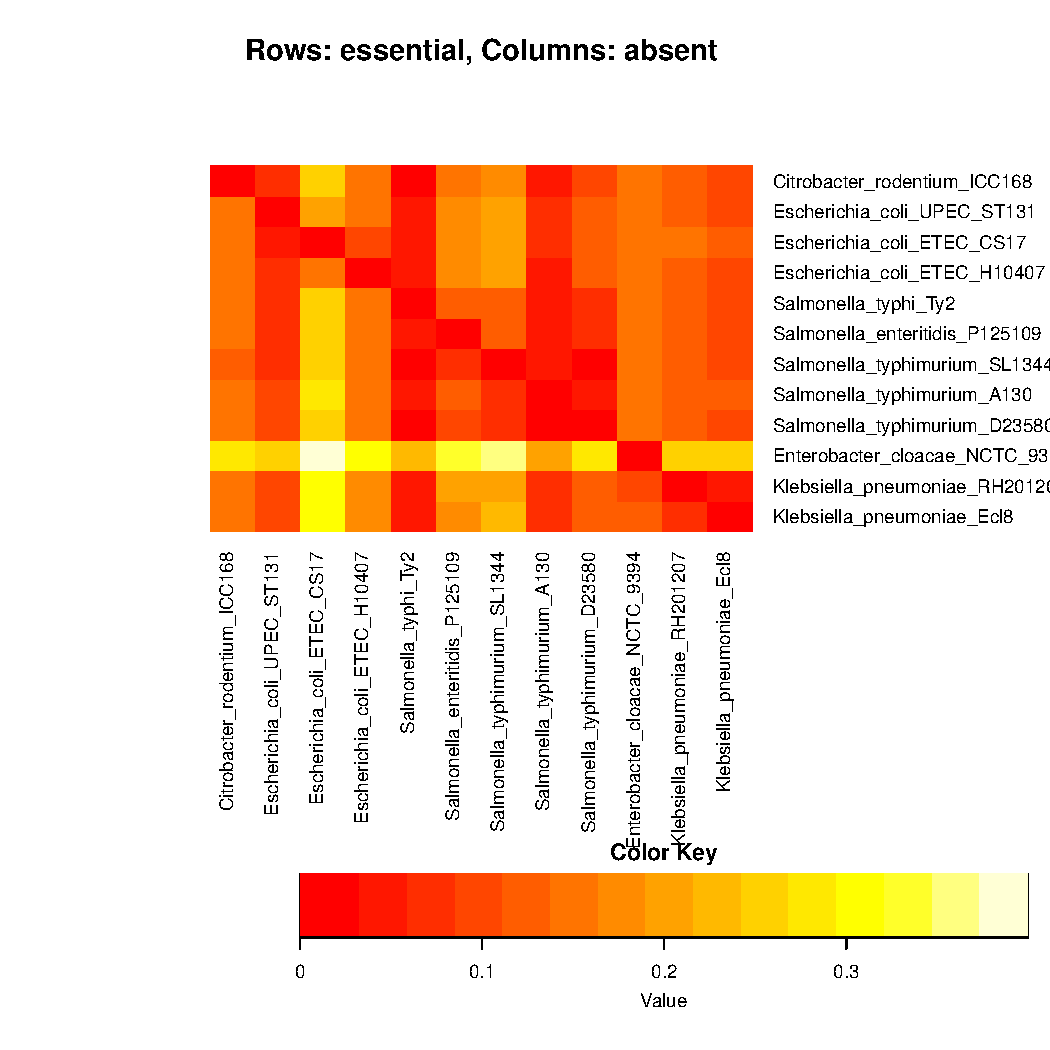
\includegraphics[page=1, scale=0.35]{essentiality-heatmap.pdf} & 
\includegraphics[page=2, scale=0.35]{essentiality-heatmap.pdf} \\
\includegraphics[page=3, scale=0.35]{essentiality-heatmap.pdf} & 
\includegraphics[page=4, scale=0.35]{essentiality-heatmap.pdf} \\
\includegraphics[page=5, scale=0.35]{essentiality-heatmap.pdf} & 
\\
\end{tabular}
\caption{The number of genes that are essential in one strain and absent in the other (upper left), the number of genes that are essential in both strains (upper right), the number of genes that are essential in one strain and present but not essential in the other strain (middle left), the number of genes that are present in one strain and absent in the other (middle right), and the number of genes that are shared between the two strains (lower left).}
\label{fig:pairwise-venn}
\end{figure*}

\section{Are conserved genes more likely to be essential?}
To find out whether conserved genes are more likely to be essential or not we have counted the number of essential, sometimes essential and never essential genes in both core and accessory genomes. The results are summarised in Table~\ref{table:core-accessory}. Core genes are the ones that have at least one copy per genome, otherwise, the genes are called accessory.

\begin{table*}[t]
\centering
\begin{tabular}{| l || c | c | c || c | c | c |}
\hline
Species&\multicolumn{3}{c ||}{Core} & \multicolumn{3}{c |}{Accessory}\\
\cline{2-7}
Name&Ess&SEss&NEss&Ess&SEss&NEss\\
\hline
Salmonella typhimurium A130&266&665&1621&53&327&1528\\
Salmonella typhimurium D23580&267&670&1624&54&339&1550\\
Salmonella typhimurium SL1344&266&674&1630&63&350&1546\\
Salmonella enteritidis P125109&266&679&1615&61&311&1015\\
Salmonella typhi Ty2&265&628&1564&56&294&1505\\
Escherichia coli UPEC ST131&299&685&1635&62&323&1767\\
Escherichia coli ETEC CS17&280&656&1603&107&356&1586\\
Escherichia coli ETEC H10407&284&656&1623&89&329&1743\\
Escherichia coli K-12&279&657&1612&174&278&1311\\
Citrobacter rodentium ICC168&304&685&1630&96&356&1868\\
Enterobacter cloacae NCTC 9394&280&623&1526&34&129&1128\\
Klebsiella penumoniae RH201207&357&864&1780&69&279&2314\\
Klebsiella pneumoniae Ecl8&357&840&1770&61&225&1751\\
\hline
\end{tabular}
\caption{The number of essential (Ess), sometimes essential (SEss) and never essential (NEss) genes in both core and accessory genomes. Core genes are the ones that have at least one copy per genome, otherwise, the genes are called accessory.}
\label{table:core-accessory}
\end{table*}

\end{document}